\documentclass{article} 

\usepackage{graphicx} % Czy musimy ręcznie dodawać pakiety? Jaki ma to sens?
%tak, automatyczne przetwarzanie dodawanych zdjęć (z folderu)
\usepackage[utf8]{inputenc}

\title{FriendBy}
\author{Mateusz Świątek, Adam Stajek, Diana Misiaczyńska, Gabriela Bułat }
\date{October 2022}

\begin{document}
\maketitle

\section{Mateusz Świątek\item \item }

Memik na dobry początek dnia (Figure~\ref{fig:altF4})

\begin{figure}[h] % kontrolowanie gdzie będzie dany element h-tutaj t-top b-bot p-next page (top) 
    \centering
    
\includegraphics[width=0.7\textwidth]{pictures/altF4.jpg} %trzeba zwiększyć współczynnik 0.2
    \caption{Tak będzie, nie zmyślam}
    \label{fig:altF4} %skrót do tego elementu
\end{figure}

% Dlaczego wyrażenie przeskoczyło do nowej linijki? bo jest \ co symbolizuje przejście do nowej linijki
\newpage


Zoba jakie fajny wzorek(Eulera): \[e^i^\pi + 1 = 0\]

a tutaj wzór na kółko
$ x^2 + y^2 = 1 $\\

W Tabeli~\ref{tab:Sudoku1} posiadasz zadanko na dziś.\\ % Do czego służy \ref{}? do odwołań do poszczególnych elementów w tym pliku


\begin{table}[h]
\centering
\begin{tabular}{|c|c|c|c|c|c|c|c|c|} % c-central r-right l-left | robi linię pomiędzy kolumnami \hline-pozioma linia
\hline
\textbf{5} & \textbf{}  & \textbf{}  & \textbf{}  & \textbf{7} & \textbf{}  & \textbf{}  & \textbf{}  & \textbf{}  \\ \hline
\textbf{}  & \textbf{3} & \textbf{}  & \textbf{}  & \textbf{}  & \textbf{9} & \textbf{}  & \textbf{2} & \textbf{8} \\ \hline
\textbf{}  & \textbf{}  & \textbf{}  & \textbf{}  & \textbf{6} & \textbf{3} & \textbf{7} & \textbf{}  & \textbf{1} \\ \hline
\textbf{}  & \textbf{}  & \textbf{}  & \textbf{}  & \textbf{}  & \textbf{8} & \textbf{2} & \textbf{}  & \textbf{}  \\ \hline
\textbf{}  & \textbf{7} & \textbf{2} & \textbf{}  & \textbf{9} & \textbf{}  & \textbf{}  & \textbf{}  & \textbf{}  \\ \hline
\textbf{9} & \textbf{}  & \textbf{5} & \textbf{}  & \textbf{}  & \textbf{}  & \textbf{}  & \textbf{7} & \textbf{6} \\ \hline
\textbf{6} & \textbf{}  & \textbf{}  & \textbf{1} & \textbf{8} & \textbf{}  & \textbf{}  & \textbf{}  & \textbf{}  \\ \hline
\textbf{}  & \textbf{1} & \textbf{7} & \textbf{9} & \textbf{3} & \textbf{}  & \textbf{6} & \textbf{8} & \textbf{4} \\ \hline
\textbf{8} & \textbf{5} & \textbf{3} & \textbf{2} & \textbf{4} & \textbf{}  & \textbf{9} & \textbf{}  & \textbf{7} \\ \hline
\end{tabular}
\caption{Takie tam zadanko - poziom EASY}
\label{tab:Sudoku1}
\end{table}\\
Wydziały na AGH
\begin{itemize}
  \item [\$] Wydział Elektrotechniki, Automatyki, Informatyki i Inżynierii Biomedycznej \verb|(Najlepszy)|
  \item [?]Wydział Inżynierii Metali i Informatyki Przemysłowej
  \item [WIET] Wydział Informatyki, Elektroniki i Telekomunikacji
  \begin{description}
     \item[Note:] Zagrożenie życia lub zdrowia
    \end{description}
  \item [\<>]Wydział Inżynierii Lądowej i Gospodarki Zasobami
  \item itd \\
\end{itemize}

Oraz najtrudniejsze przedmioty:
\begin{enumerate}
  \item Analiza \texttt{Matematyczna}
  \item Algebra Liniowa i Geometria analityczna 
  \item Podstawy Programowania
  \item WF
\end{enumerate}
\newpage

\begin{center}
\resizebox{!}{0,85cm}{Hobbit}\\
\end{center}

{\huge W} pewnej norze ziemnej mieszkał sobie pewien \textbf{hobbit} . Nie była to szkaradna, brudna, wilgotna nora, rojąca się od robaków i cuchnąca błotem, ani też sucha, naga, piaszczysta nora bez stołka, na którym by można usiąść, i bez dobrze zaopatrzonej spiżarni; była to nora hobbita, to znaczy: nora z wygodami.

Miała drzwi \underline{doskonale} okrągłe jak okienko okrętowe, pomalowane na \textbf{\textit{zielono}},
z lśniącą, żółtą mosiężną klamką, sterczącą dokładnie pośrodku. Drzwi prowadziły do hallu, który miał kształt rury i wyglądał jak \emph{tunel}: był to bardzo wygodny
tunel, nie zadymiony, z boazerią na ścianach i chodnikiem na kafelkowej podłodze; nie brakowało tu politurowanych krzeseł ani mnóstwa wieszaków na kapelusze i płaszcze, bo hobbit bardzo lubił gości. Tunel wił się w skrętach, wił się i wił,
wdrążając się głęboko, choć wcale nie prostą drogą, we wnętrze pagórka — a raczej: Pagórka, bo tak go nazywano w promieniu wielu mil — a mnóstwo okrągłych drzwiczek otwierało się to po jednej, to po drugiej jego stronie. Hobbici nie
uznają schodów. Sypialnie, łazienki, piwnice, spiżarnie (mnóstwo spiżarni!), garderoby (hobbit miał kilka pokoi przeznaczonych wyłącznie na ubrania), kuchnie,
jadalnie — wszystko mieściło się na tym samym piętrze, a nawet wzdłuż tego samego korytarza. Najparadniejsze pokoje znajdowały się z lewej strony, (patrząc
od wejścia), ponieważ tylko te miały okna, głęboko osadzone, okrągłe okna z widokiem na ogród, a dalej na łąki zbiegające w dół ku rzece. 

\vspace{2cm}
Bilbo razem z Gandalfem zrobią za nas projekt, dalsza historia nastapi za rok:  % Do czego służy input? służy do wstawiania "kodu" z innych miejc w projekcie
wprowadzone zmiany z githuba
i jeszcze z komputera ;)
i na samym końcu z Overleafa.

\section{Adam Stajek\item \item }
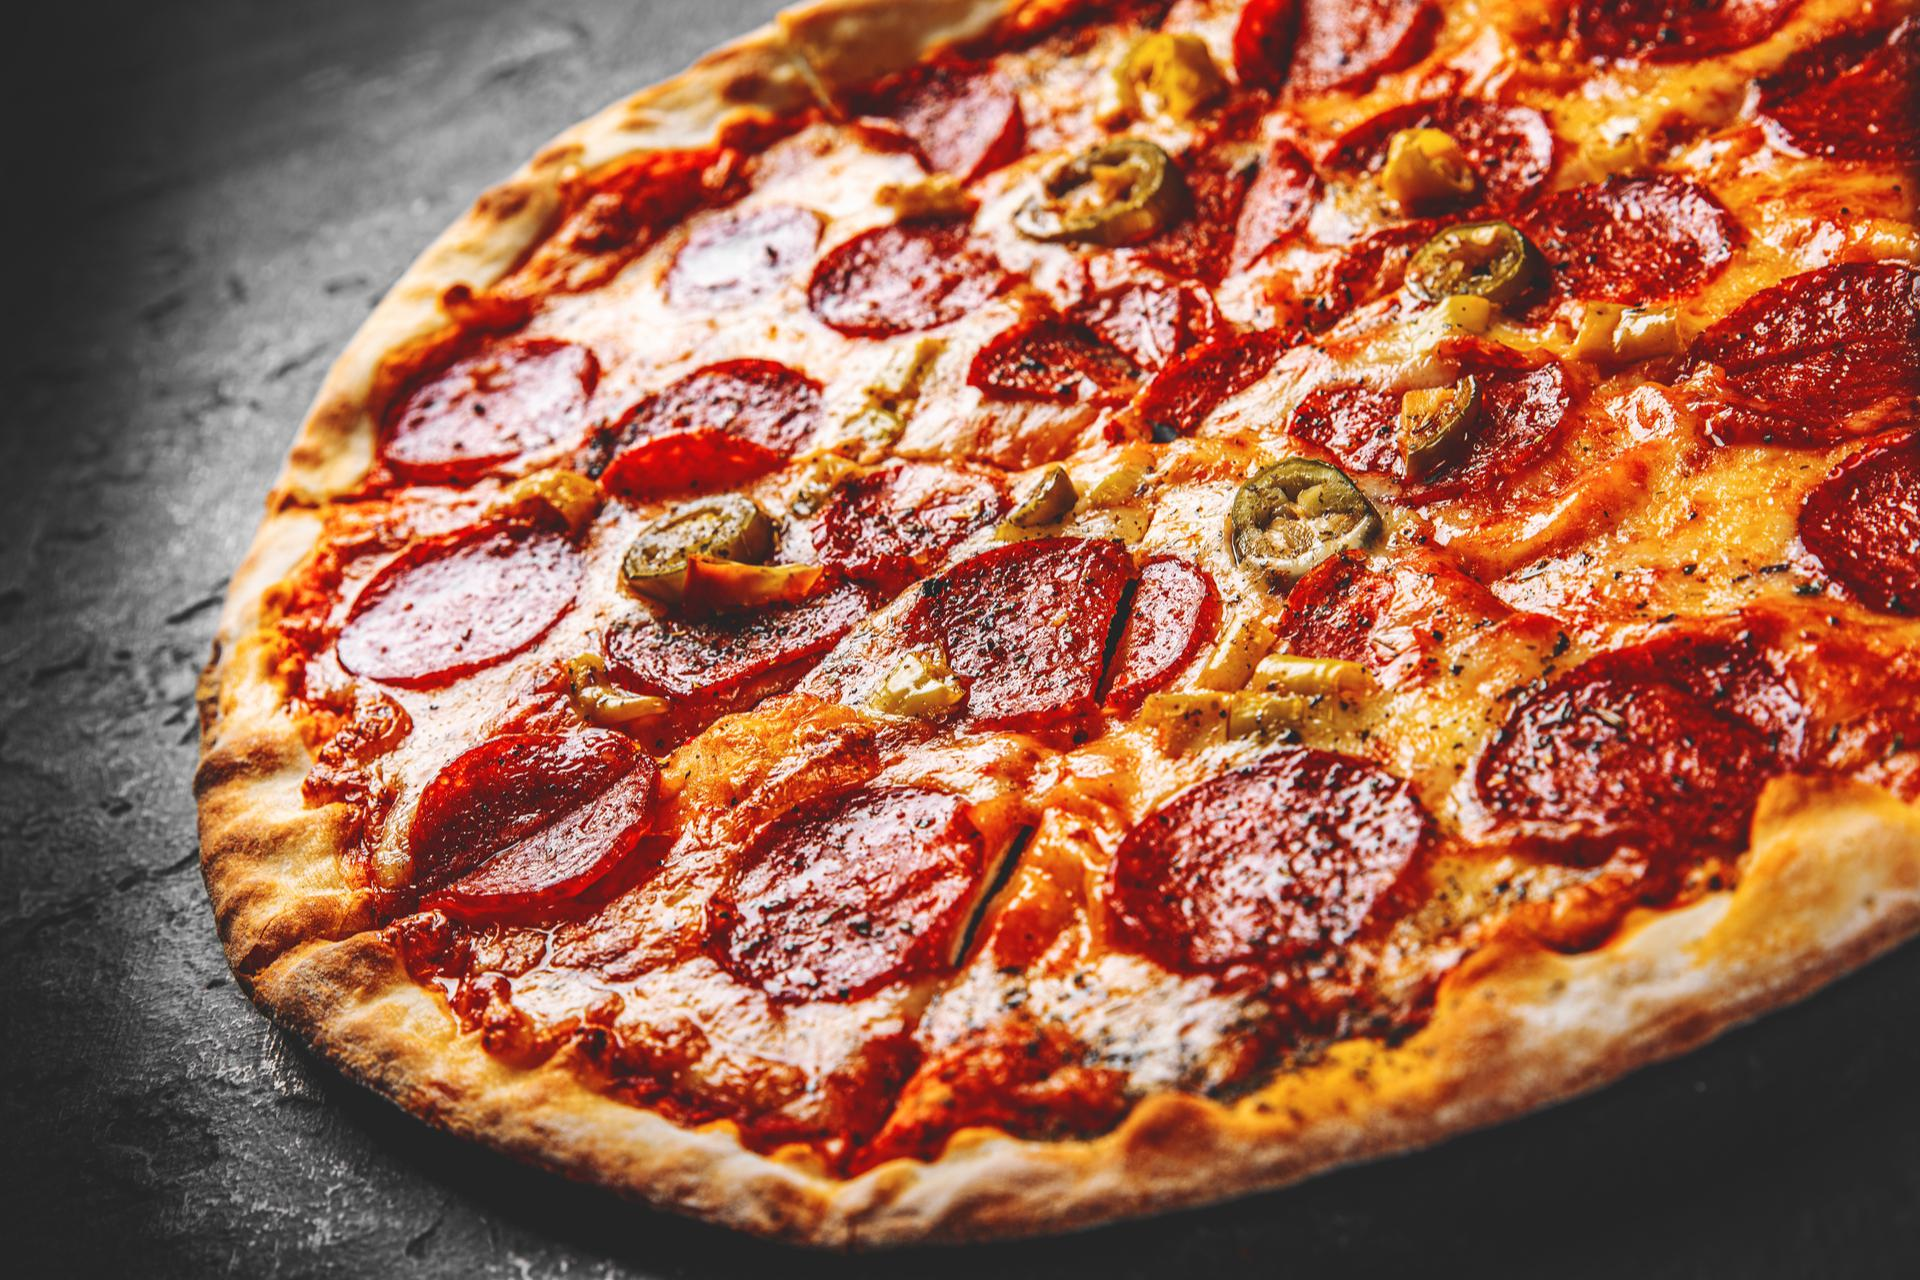
\includegraphics[width=5cm, height=4cm]{pictures/pizza.jpg} 
\newline
wzór na obliczenie pola pizzy: \(P= \pi r^2\)
\newpage
Kocham:
\begin{itemize}
  \item AGH
  \item Samogłoski
  \item Informatykę
\end{itemize}
Nie kocham:
\begin{enumerate}
  \item Pizzy z ananasem
  \item Ostrowca Świętokrzyskiego
  \item Staszica
\end{enumerate}

\newline

\begin{table}
\label{tabela}
\begin{tabular}{|l|l|l|l|l|}
\hline
a & b & c & d & e \\ \hline
f & g & h & i & j \\ \hline
k & l & m & n & o \\ \hline
p & t & d & t & u \\ \hline
\end{tabular}
\end{table}

Studia na kierunku \textbf{Informatyka i systemy inteligentne} wyposażają w wiedzę i praktyczne umiejętności z zakresu informatyki oraz sztucznej inteligencji i przygotowują do tworzenia i projektowania rozwiązań informatycznych wykorzystujących i integrujących różne systemy inteligentne. W programie studiów uwzględniono przedmioty informatyczne, matematyczne oraz fizyczne. Kształcenie na tym kierunku to jednak głównie przedmioty związane z programowaniem, a także \underline{inżynierią oprogramowania}. \par Student zdobywa kompetencje dotyczące języków i technik programowania, algorytmiki, złożoności obliczeniowej, baz danych, analizy danych oraz analizy procesów biznesowych. Przygotowuje się do projektowania, testowania i wdrażania systemów informatycznych, budowy interfejsu użytkownika, systemów operacyjnych oraz sieci komputerowych. Poznaje także takie zagadnienia, jak uczenie maszynowe, sztuczna inteligencja, programowanie inteligentnych systemów wbudowanych oraz projektowanie złożonych systemów informatycznych, co w efekcie pozwala mu na realizację zadań związanych z \emph{wytwarzaniem oprogramowania}. \newline
\newline
Pamiętaj o tabeli na stronie \pageref{tabela} \newline

\input{chapters/chapter3_GabrielaBułat}

\input{chapters/chapter4_DianaMisiaczyńska}



\end{document}
